\documentclass[a4paper,10pt]{article}
\usepackage[utf8]{inputenc}
\usepackage[margin=0.5in]{geometry}
\usepackage{graphicx}
\usepackage{amsmath}
\usepackage{hyperref}

%opening
\title{Breakdown of Asteroid Detection and Identification System}
\author{J.G.P. Vermeulen}

\begin{document}

\maketitle
\begin{figure}[h!]
\centering
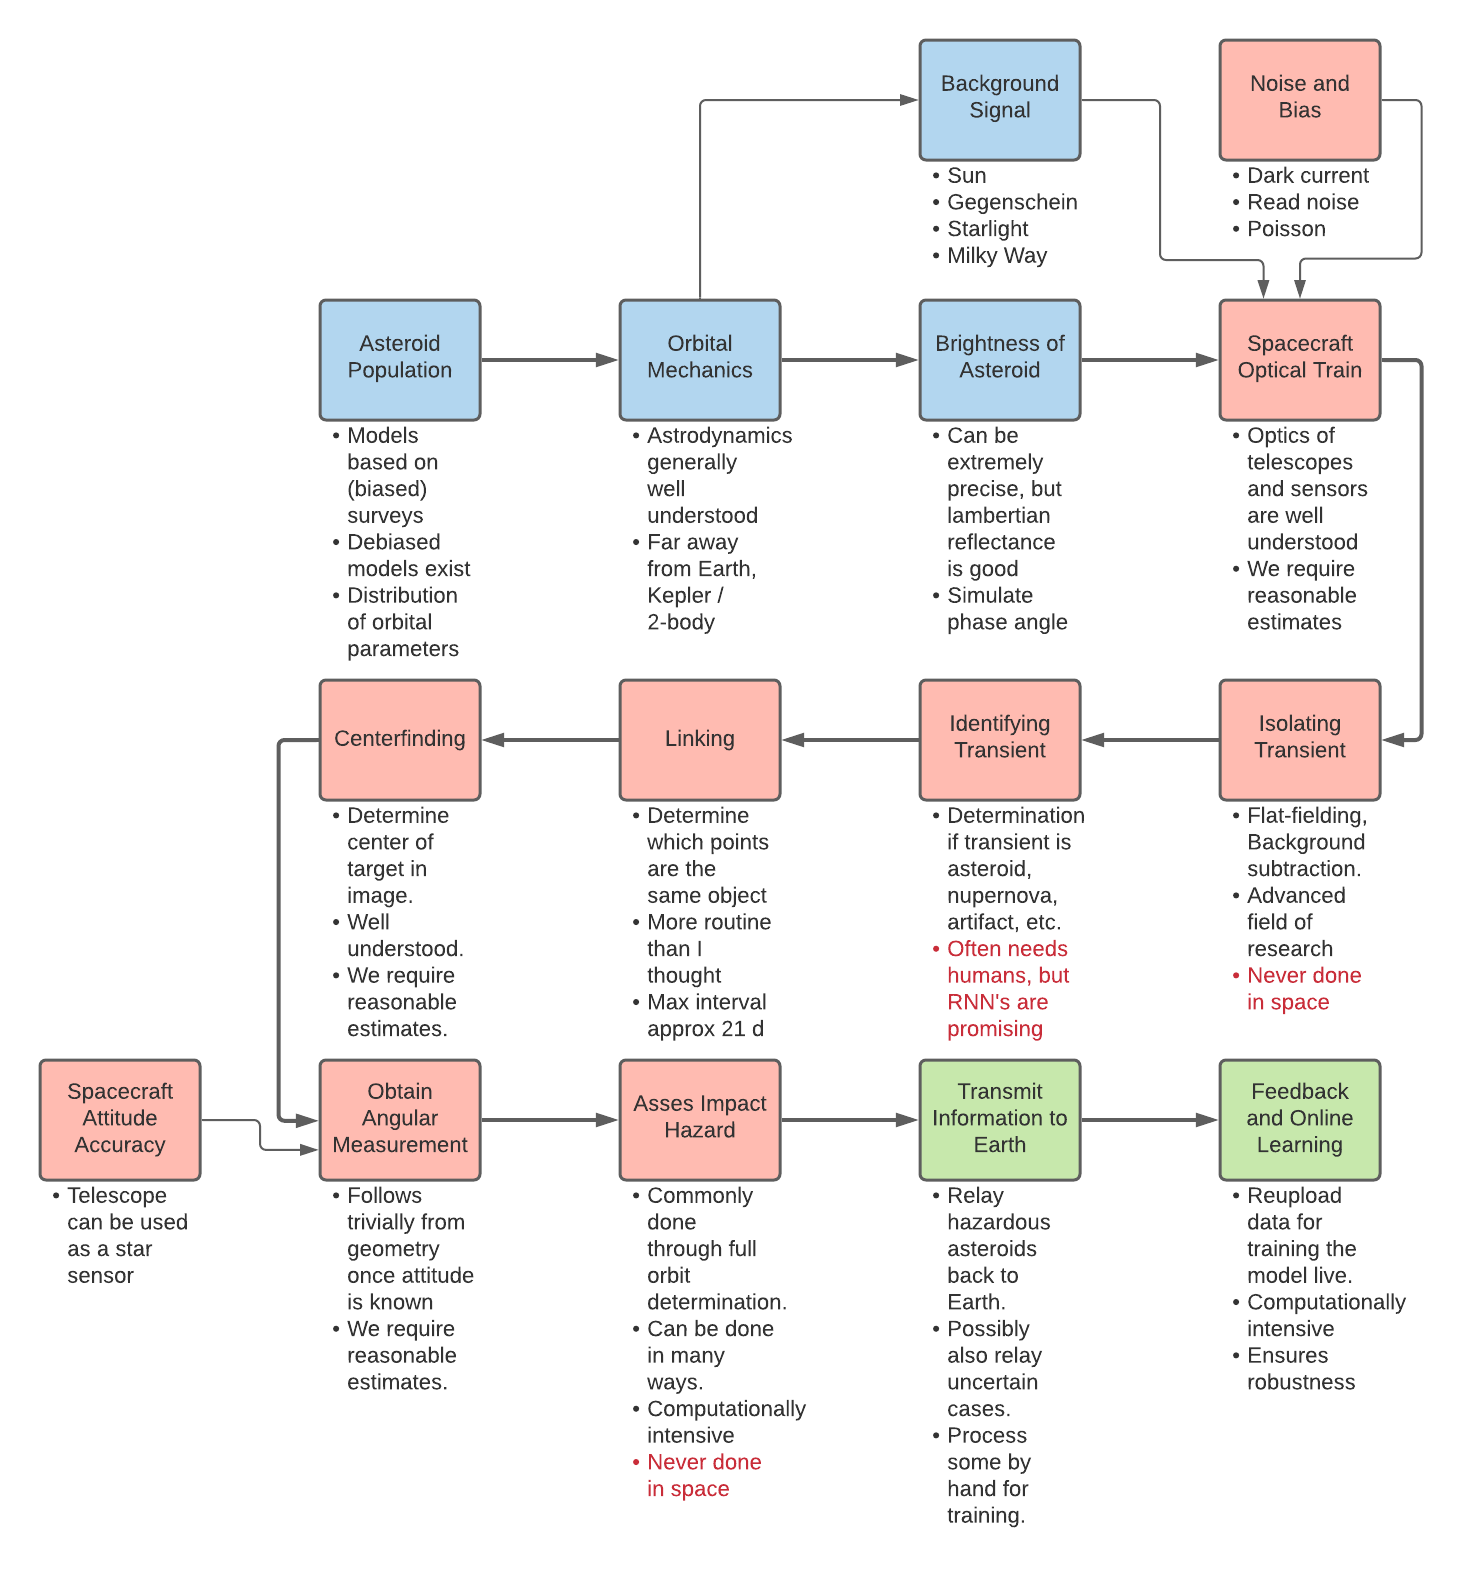
\includegraphics[width=1.0\textwidth]{functional_flow.png}
\caption{Functional Flow Diagram of the System. Blue = Space, Red = Satellite, Green = Earth. Red text indicates a knowledge gap.}
\label{fig:FFD}
\end{figure}
\newgeometry{top=1.5in, bottom=1.2in, left=1.2in, right=1.2in}
\section{Explanation of the System}
\autoref{fig:FFD} shows a functional flow diagram of the complete detection system, as seen from a research standpoint. Marked in blue are processes going on in space, in red are processes in the spacecraft, and in green are processes on Earth. Topics marked in red present knowledge gaps. They will be treated separately below, with references to the state-of-the-art in the relevant research field where applicable. But first, the mission of the system will be stated: \textit{to reduce risk to human life and property by assessing previously unidentified NEA's for impact hazard}. Current NEA survey completeness is highly limited by the location of the surveys (all surveys are carried out from Earth or Earth orbit). This opens up the problem of asteroids being too distant from Earth at a similar semi-major axis (which conversely lowers their impact risk, because of the very long time to impact), objects having a very long period (very small observation windows, but this problem is hard to resolve), or objects which are too close to the Sun to observe, or in resonant orbits. Several authors have suggested using a satellite system which is not in Earth orbit for this, such as in a Venusian orbit. Most influential among these is the work of Stokes et al.(2017)\footnote{Stokes, G. H. et al. (September 2017): ``Update to Determine the Feasibility of Enhancing the Search and Characterization of NEOs'' Tech. Rep. \textit{NASA JPL CNEOS}}. There is however an important problem with such missions: The communications rate will be severely limited, in worst cases down to 5 kpbs (see Stokes et al.(2017), page 84). This makes it impossible to transmit the terabytes of images generated daily without using very strong compression. In turn, this compression will destroy the required detail to spot extremely faint objects. \textbf{Therefore, on-board processing is mandatory}.

\section{Asteroid Population}
Models of asteroid populations are mainly based on existing NEA surveys, such as Harris and D'Adbramo (2015)\footnote{Harris, A. W. and D'Abramo, G. (2015): ``The Population of Near-Earth Asteroids'' \textit{Icarus, 257}.} and the results of the NEOWISE mission presented by Mainzer et al. (2012)\footnote{Mainzer et al. (2012): ``Characterizing Subpopulations within the Near-Earth Objects with NEOWISE: Preliminary Results'' \textit{The Astrophysics Journal, 752}}. The issue with these models is obvious: As they are based on existing NEA surveys, which have all been performed from Earth, they are affected by the same biases. However, debiased models exist, such as the one presented by Bottke et al. (2001)\footnote{Bottke, W. F. et al. (2001): ``Debiased Orbital and Absolute Magnitude Distribution of the Near-Earth Objects'' \textit{Icarus, 156}}. These models specify a distribution of orbital parameters, which can be used to generate an asteroid population and simulate a survey. This approach is taken by other authors, including Stokes et al. (2017). The simulation can be verified by running experiments on existing catalogs of NEA's.

\section{Orbital Mechanics}
Orbital mechanics is generally a well-understood problem. The required precision for assessing impact hazard years into the future is not extremely large. Therefore, no interesting research opportunities are present in this field and application. The secondary question is the level of detail required for accurate simulation. As we are not interested in the precise orbit, a simple keplerian formulation of the orbit should suffice if the target is sufficiently far away from Earth. However, as a special type of target of interest are asteroids in a resonance with Earth and Venus, a more complex formulation would be required. These formulations are readily available (e.g. Curtis, Wakker).

\section{Signal of Background and Signal of Asteroid and Noise and Bias}
A complicating factor in the analysis is the background signal and various noise terms. In general the background signal is caused by the Sun, reflections off interplanetary dust, and the background starlight (which is more intense in the galactic plane). Noise is generally a combination of sensor technology and poisson noise. It is possible to model all these terms individually, as they are well described (see e.g. Owen Jr. (2015)\footnote{Owen, Jr. W. M. (2017): ``Methods of Optical Navigation''. \textit{AAS/AIAA Space Flight mechanics Meeting, 11-215}}), but most authors (see e.g. Stokes et al. (2017), page 111-113) seem to suffice with a calculation of signal-to-noise ratio. An interesting component of this equation is the phase angle, which effectively limits the observations to within ~90 degrees of opposition, although this is no hard limit.

\section{Spacecraft Optical Train}
The functioning of telescopes and modern sensors is well understood (see Owen, Jr. (2015)), and any improvements would be more in the field of optics or sensor electronics. See the previous section for how to account for the imperfections.

\section{Isolating Transients}
Also known as ``Source extraction'', the next problem presents the first (limited) research opportunity. Transient isolation is performed by a process consisting of (in essence) camera calibration and background subtraction. This is generally a tricky thing to do: images taken in space are filled with stars, galaxies, nebulas, etc. and camera noise can be a real problem for faint targets. Vermeulen (2021)\footnote{Vermeulen, J. G. P. (2021): ``Identification of Impact-Hazardous Asteroids: Literature Study'' \textit{TU Delft} (unpublished)} gives an \textit{excellent} explanation of the various techniques, possibilities and algorithms that have been developed over the years (there are too many to cite here). However, there is an important gap for the mission: As stated by Stokes et al. (2017), these techniques have never been succesfully demonstrated in-flight. Data always had to be transmitted back to Earth for processing, which as we stated previously, is undesirable. \textbf{Therefore, in-flight source extraction presents a knowledge gap.} Can this be done more efficiently from space?

\section{Identifying Transients}
After image differencing has removed all the ``static'' sky objects, only the ``transients'' are left. These transients are not necessarily only asteroids: they can also be distant supernovae, variable stars, or simply cosmic ray hits or electric artifacts in the detector. Classifying these events traditionally required a lot of human intervention, but some new techniques based on light-curve analysis have emerged over the past years. These still suffer from problems with computational intensity and image alignment. New techniques have emerged in this field using (C)RNN's, which have been showing very promising results (See e.g. Cassaco-Davis et al. (2019)\footnote{Cassasco-Davis, R. et al. (October 2019): ``Deep Learning for Image Sequence Classification of Astronomical Events'' \textit{Publications of the Astronomical Society of the Pacific, 131}} and other papers by the same author). This is also still a very novel field, and although it is gaining in popularity, it still has openings for further research. Additionally, it has also not been done in-flight. However, this topic is not entirely algined with our expertise, I think.

\section{Linking}
Linking refers to solving the question which transients on subsequent images belong to the same object, or, when using multiple satellites, which transients on the different images at the same time belong to the same object. Although this might seem difficult, no authors indicate difficulty with it, if the observations are close enough together. This topic was greatly improved by the work of Milani et al. (2004)\footnote{Milani, A. et al. (April 2004): ``Orbit Determination with Very Short Arcs: I. Admissible Regions'' \textit{Celestial Mechanics and Dynamical Astronomy, 90}} and subsequent papers. Their work allows for computing the possible parameter space of an asteroids orbit. This space can then be used to link the observation to other observations far away from it in time, or even before it (known as ``precovery''). Note, however, that this is a computationally very intensive process, and thus unsuited for in-flight usage.

\section{Centerfinding and Obtaining Angular Measurements}
With the transients located in the images, the image data needs to be processed into an angular observation. To do this, first the center is computed (which can be done at sub-pixel accuracy), and then the coordinates in the image are translated into angular measurements using information from the spacecraft attitude. These are well-described processes, see Owen, Jr. (2017) for a full explanation of the process. An interesting new development here is using the survey telescope itself as a star sensor, something which is demonstrated succesfully by the Canadian NEOSSat mission.

\section{Asses Impact Hazard}
With sets of measurements of the same target obtained, there is only one thing left to do: asses the impact hazard. There are several approaches to this. Firstly, when a survey attempts to catalogue objects, it will want to do a full orbit specification. The methods for doing this are still largely based on Gauss' Method (see Curtis for a derivation). \textbf{However, there is discrepancy in literature with regards to the required length of observation:} for example, Der (2012)\footnote{Der, G. J. (2012): ``New Angles-only Algorithms for Initial Orbit Determination'' \textit{Advanced Maui Optical and Space Surveillance Technologies Conference}} indicates a timespan of ``days to months'', worsening for objects with little relative motion to the observer (such as those in a near-Earth orbit. On the other hand, Stokes et al. (2017), page 102, mention only requiring three nights of observation in a 21 day period to perform full orbit determination, calling it ``routine''. In addition, they mention the linking to become a problem after 21 days. Therefore, the question of how difficult this is, is hard to answer. However, there is still a tangible problem here. As Gronchi (2004)\footnote{Gronchi, G. F. (2004): ``Classical and Modern Orbit Determination for Asteroids'' \textit{Proceedings of the IAU, 196}} mentions, it is sometimes hard to link tracklets from night to night effectively (which again constrasts with the earlier view that linking is a routine operation). \textbf{Therefore, there are two openings for research here: Firstly, a space-based system can image the same part of the sky constantly, eliminating the linking problem. Secondly, a multiple-satellite system might be able to do orbit determination with a vastly shorter set of data}.\newpage

The second method of impact hazard assessment relates to the ``warning'' approach. Here, our efforts are not focussed on catalogueing all objects. Instead, we simply need to warm Earth about the danger. In this case, full orbit determination is unneccessary (and thus less observations suffice). Therefore, we might also compute different metrics, such as the MOID. If the object has a MOID below a certain threshold, we send some information about our observations to Earth, where it will be further processed (perhaps with a precovery). Furthermore, we could even treat this as a one-class classification problem. In this case, we are not concerned with the targets orbit at all. We simply construct a machine learning or neural network application which classifies a set of measurements as belonging to a impact-hazardous object, or not. In terms of effectiveness of the machine learning solution, this would present an even better alternative, as the exact MOID is irrelevant, and thus we require less data for training. In addition, it allows tweaking the precision/recall relation. \textbf{However, this is not the normal way to perform these kinds of surveys. As such, it will be harder to justify the choice of metric; why aren't we just performing orbit determination?} This approach would be more suited to a single-satellite approach.\\

Regardless of the decision, there is another research opportunity here. Some of the algorithms can be computationally intensive, and they have today never been carried out in a deep space mission, such as the ones proposed at Venus.

\section{Tranmission to Earth for Processing and Re-upload for Online Learning}
With the information obtained in the last step, this information can be transmitted to Earth. This opens up several interesting possibilities: For example, only specific data on ``flagged'' hazardous asteroids could be transmitted. This allows using the limited downlink capacity for just important data. In case of full orbit determination, we could just transmit orbital elements. In case some objects have a high uncertainty, the data could be downlinked to Earth, analysed in more detail, and then re-uploaded as labelled data to the spacecraft to carry out online learning of the system. The latter is a rather expensive operation, computationally, but it is well documented and offers some amazing opportunities for implementation of the research in practice.

\section{Conclusion: Where to Contribute}
Lastly, a short summary of the intersection of knowledge gap and usefulness. In other words: Where can the planned research contribute? As identified, there is desire for a space system that does not orbit Earth, to identify hazardous asteroids and/or catalogue them. The missing pieces of the puzzle are:
\begin{itemize}
 \item A way of performing source extraction / transient identification that can be done in-flight. 
 \item Better, or more efficient, ways of identifying transients. However, a lot of work has already been done on this topic.
 \item Ways to asses impact hazard from angular measurements in-flight from limited observations. Note that the scope of this problem is badly defined due to the previously mentioned discrepancies in literature.
 \item Ideally, a full system capable of doing the full circle, autonomously, from deep space. Perhaps, using a spacecraft formation and multiple images at different angles, or using ANN's??
\end{itemize}

\end{document}
